%----------------------------------------------------------------------------------------
\begin{document}
% This declaration makes TeX less fussy about line breaking.
% This can prevent overfull boxes, but may leave too much space between words.
\sloppy
\pagenumbering{gobble}  % remove page numbers (and reset to 1)
\clearpage

%----------------------------------------------------------------------------------------
%       TITLE SECTION
%----------------------------------------------------------------------------------------
% Place title on the separate page
% maketitle
\title{Шаблон документа для LuaLaTeX}
\author{Николай Якуба\\nick.yakuba@gmail.com}
\date{2018}

\maketitle
\thispagestyle{empty}  % remove any header and footer (including page number)

%----------------------------------------------------------------------------------------
% titlepage
\begin{titlepage}
  \begin{center}
    Министерство образования и науки Российской Федерации\\
    Санкт-Петербургский политехнический университет Петра Великого\\
    Высшая школа программной инженерии\\
  \end{center}
  \vspace{0.3\textheight}

  \begin{center}
    {\Huge Название работы}\\
    \vspace{0.05\textheight}
    \begin{tabular}{lll}
      & \hspace*{0.3\textwidth} & \\
      Выполнил & & \\
      студент гр. 12345& &Н.В. Якуба\\[0.5em]
      Руководитель & & \\
      к.т.н, доцент & & П.В. Трифонов\\
    \end{tabular}
    \vfill
    Санкт-Петербург\\
    \the\year 
  \end{center}
\end{titlepage}


%----------------------------------------------------------------------------------------
\cleardoublepage  % start actual document from the odd page
\newgeometry{left=10mm,right=30mm,top=20mm,bottom=20mm}  % set page margins
%\fontdimen2\font=0.25em  % set minimum inter word space
%\setstretch{1.5}  % set line spacing 

\pagestyle{plain}  % restore default footer with page number
\pagenumbering{arabic}  % restore page numbers (alatexnd reset to 1)
\setcounter{page}{2}  % set first page number = 2

%----------------------------------------------------------------------------------------
%       ABSTRACT
%----------------------------------------------------------------------------------------
\begin{abstract}
  Данный документ является шаблоном, который может быть использован для создания отчетов, статей и других документов.

  Файл {\em main.tex} содержит общие настройки шаблона, а также список используемых пакетов.
  Файл {\em title.tex} используется для описания титульного листа.
  Текст документа, тестирующий возможности используемых расширений, находится в файле {\em document.tex}.
\end{abstract}

%----------------------------------------------------------------------------------------
%       TABLE OF CONTENTS
%----------------------------------------------------------------------------------------
\setcounter{tocdepth}{3}  % use at most 3 levels in table of contents
\hypertarget{contents}{}  % set anchor for link to contents from footer
\tableofcontents
\clearpage

%----------------------------------------------------------------------------------------
%       BODY OF THE DOCUMENT
%----------------------------------------------------------------------------------------
\section{Введение}
TeX --- это система компьютерной верстки, разработанная американским профессором информатики Дональдом Кнутом в 1978.
Вместе с языком описания шрифтов Metafont TeX был предназначен для быстрого создания документов высокого качества, а также для предоставления инструментов, дающих одинаковый результат на всех компьютерах.

LaTeX является надстройкой над TeX, включающей в себя огромное число макросов и расширений, упрощающих создание документов.
LuaLaTeX в свою очередь расширяет возможности LaTeX, предоставляя поддержку unicode и интегрируя язык Lua для создания сложных расширений.

%----------------------------------------------------------------------------------------
\subsection{Hello, world!}
Самый базовый документ приведен на рисунке \ref{f1}.
Документ начинается с указания его типа.
В данном случае это {\em article}.
Текст документа должен быть заключен между {\textbackslash}begin\{document\} и {\textbackslash}end\{document\}.
Число пробелов в строке не влияет на ее отображение.

\begin{figure}[b]  % display figure in the [b]ottom of the page
  \centering
\begin{verbatim}
\documentclass{article}
\begin{document}
This is my \emph{first} document prepared in \LaTeX.
\end{document}
\end{verbatim}
\caption{Пример документа}
\label{f1}
\end{figure}

Текст разделяется на абзацы.
Для перевода текста на новую строку можно использовать макрос '{\textbackslash}{\textbackslash}'.
Ниже слева приведен код TeX, а справа --- его отображение в документе.
\begin{multicols}{2}
\begin{verbatim}
Дефис: какой-то.

Новый абзац.\\
Перенос. Интервал 10 -- 15.

Это предложение --- текст,
в котором есть тире.
\end{verbatim}
  \columnbreak
Дефис: какой-то.

Интервал 5 -- 10.\\
Интервал 10 -- 15.

Это предложение --- текст,
в котором есть тире.
\end{multicols}

Более подробное введение можно прочитать в \cite{latexWikibook}.

%----------------------------------------------------------------------------------------
\section{Возможности TeX}
\subsection{Титульный лист и оглавление}
Существует несколько способов сформировать титульный лист.
Первый способ --- использовать команду '{\textbackslash}maketitle'.
Перед ее вызовом необходимо указать название работы, перечислить авторов, а также указать дату.

Второй способ заключается в создании отдельной страницы.
Для ее создания используется окружение {\em titlepage}.

Для создания оглавления используется команда '{\textbackslash}tableofcontents'.

Подробнее см. \cite{latexTitle,latexTOC}

%----------------------------------------------------------------------------------------
\subsection{Списки}
Существует 2 типа списков:
\begin{enumerate}
\item Нумерованный список (окружение {\em enumerate})
\item \label{item2}
  Ненумерованный список (окружение {\em itemize})
\end{enumerate}

Каждый элемент списка начинается с команды '{\textbackslash}item', нумерация осуществляется автоматически.
На элементы списка можно ссылаться.
Ниже приведен пример списка \ref{item2}.

\begin{itemize}
\item первый тезис
\item второй тезис
\item третий тезис
\end{itemize}

Подробнее о списках можно прочитать в документации \cite{latexLists}.

%----------------------------------------------------------------------------------------
\subsection{Вставка рисунков и таблиц}
Для вставки рисунков предусмотрено окружение {\em figure}, а для вставки таблиц --- окужение {\em table}.
Рисунок \ref{f2} и таблица \ref{t1} являются простыми примерами использования указанных окружений.
Подробнее см. \cite{latexFigures,latexTables}.

\begin{table}
  \centering
  \caption{Пример таблицы}
  \begin{tabular}{|l || c  r|}
    \hline
    left & center & right\\
    \hline
    1 & 2 & 3\\
    Awesome & text & \\
    \hline
  \end{tabular}
  \label{t1}
\end{table}

\begin{figure}
  \centering
  \includegraphics[width=0.3\textwidth]{./plots/eps/{96}{40}_normal.eps}
  \caption{График из gnuplot}
  \label{f2}
\end{figure}

%----------------------------------------------------------------------------------------
\subsection{Вставка математических формул}
Математические формулы могут быть встроены в текст, например $E = mc^2$, или вынесены на отдельную строку.
\begin{equation} \label{eqM}
  M = \begin{pmatrix}1&0\\1&1\end{pmatrix}
\end{equation}

Доступные математические шрифты приведены на рисунке \ref{f3}.
Ссылки на формулы также формируются автоматически, например, формула \eqref{eqM}.
Подробнее про вставку и редактирование формул см. \cite{latexMath}.

\begin{figure}
  \centering
  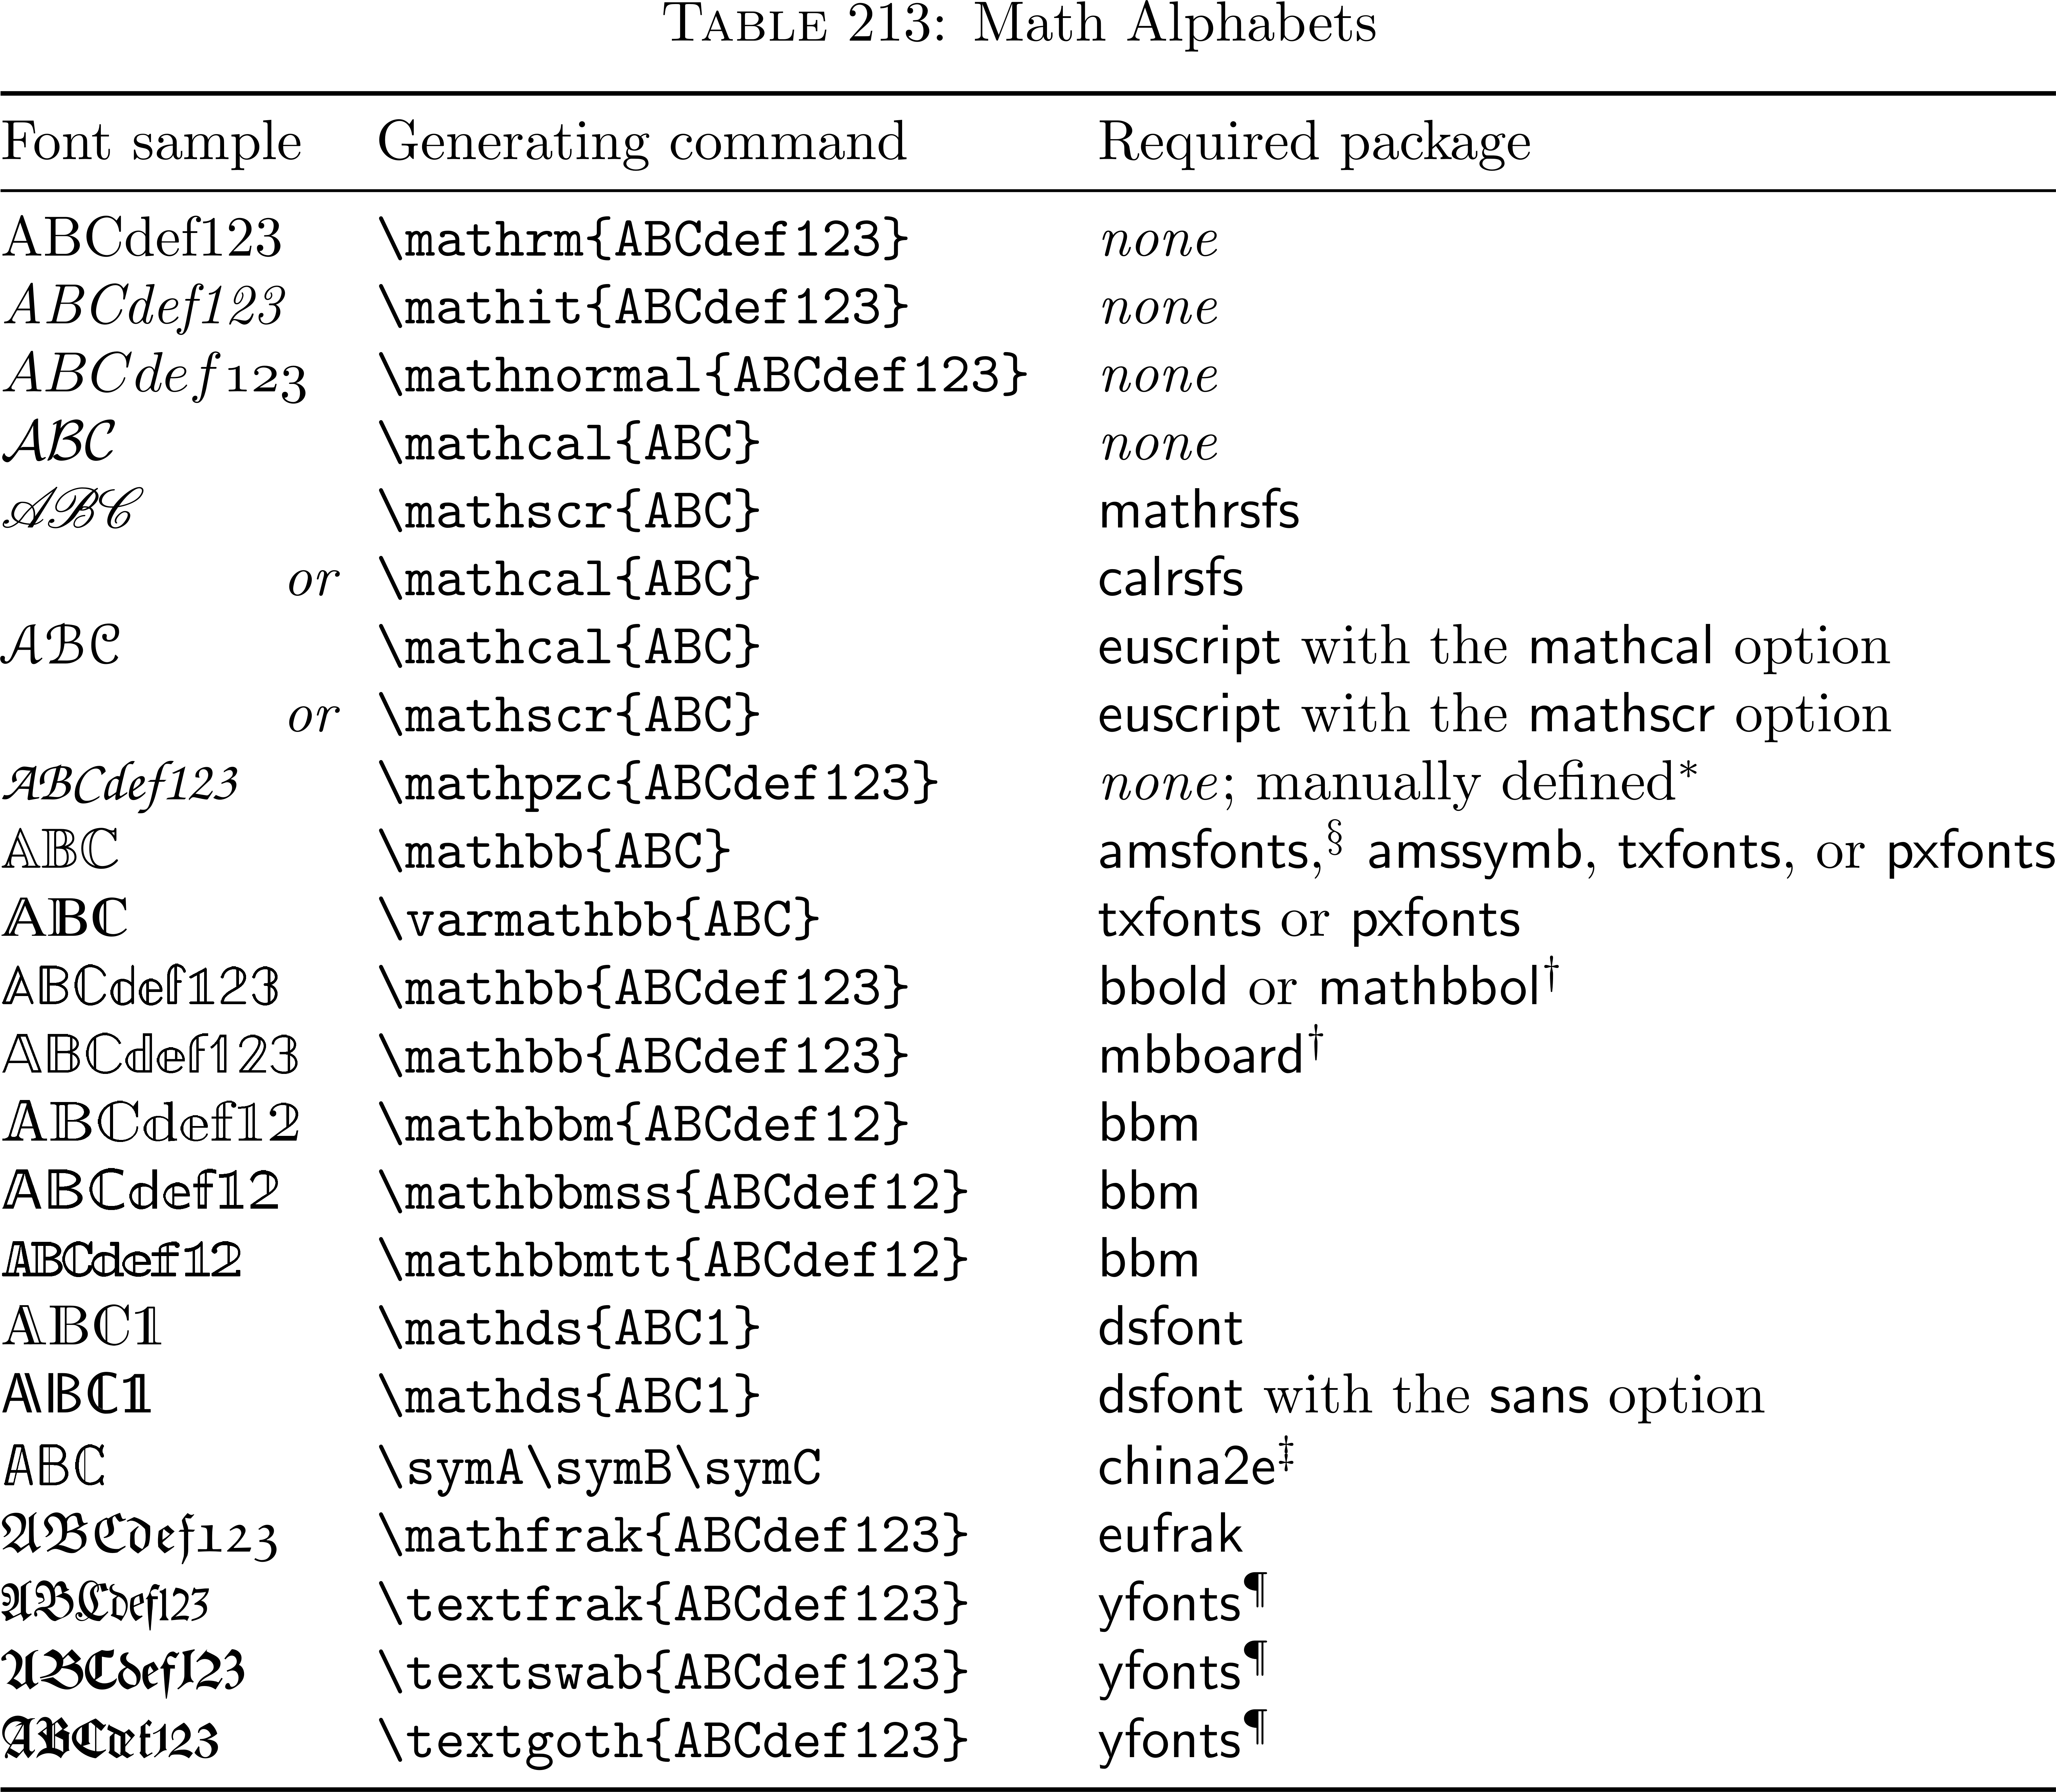
\includegraphics[width=0.5\textwidth]{mathAlph.png}
  \caption{Доступные математические шрифты}
  \label{f3}
\end{figure}

Выравнивание по знаку равенства:
\begin{align}
  \begin{split}
    S &= 1 + 2 + \dots + n - 1 + n =\\
      &= \frac{1 + n}{2}n
  \end{split}
\end{align}

%----------------------------------------------------------------------------------------
\subsection{Список литературы}
Список литературы формируется автоматически, и может быть явно указан в конце документа.
Пример явного формирования списка литературы приведен ниже:\\[1em]

\begin{minipage}{\linewidth} % prevent page break inside verbatim environment
\begin{verbatim}
\begin{thebibliography}{9}
\bibitem{lamport94}
  Leslie Lamport,
  \textit{\LaTeX: a document preparation system},
  Addison Wesley, Massachusetts,
  2nd edition,
  1994.
\end{thebibliography}
\end{verbatim}
\end{minipage}\\[1em]

Другой способ формирования списка литературы заключается в использовании BibTeX.
Команда {\em addbibresource} указывает файлы, содержащие перечень работ, на которые могут быть сделаны ссылки в статье.
Фактически, данные файлы формируют локальную базу данных, содержащую информацию о литературных источниках.
Пример записи приведен ниже:\\[1em]

\begin{minipage}{\linewidth} % prevent page break inside verbatim environment
\begin{verbatim}
@article{zinoviev1976generalized,
    author = {В.А. Зиновьев},
    title = {Обобщенные каскадные коды},
    journal = {Проблем передачи информации},
    year = {1976},
    volume = {12},
    issue = {1},
    pages = {5--15}
}
\end{verbatim}
\end{minipage}\\[1em]

После этого имя {\em zinoviev1976generalized} может быть использовано для создания ссылки командой {\em cite}.
Подробнее о BibTeX см. \cite{latexBib}.

%----------------------------------------------------------------------------------------
\clearpage
\section{Используемые пакеты}
\subsection{multicols}
Пакет предоставляет возможность размещать текст в нескольких столбцах.
Распределением текста по столбцам можно управлять командой {\em columnbreak}.

Альтернативныый способ создания нескольких колонок текста --- использование окружения {\em minipage}, который позволяет более гибко настраивать параметры столбцов.

\begin{multicols}{3}
В настоящее время разработаны алгоритмы построения и декодирования полярных кодов, обладающие приемлемой сложностью, и демонстрирующие низкую вероятность ошибки декодирования для заданной скорости кода.
Однако, современные системы связи также предъявляют жесткие требования к времени обработки принятого сообщения, которое характеризуется величиной задержки декодирования.

В данной работе ставится задача разработки методов и кодовых конструкций, позволяющих уменьшить задержку списочного алгоритма декодирования полярных кодов.
В работе предложено два различных подхода к снижению задержки декодирования полярных кодов.
Один из подходов заключается в использовании метода, позволяющего завершить декодирование заведомо неправильных кодовых слов. \todo{Подробнее}
Такие методы называют методами раннего останова.
Другая часть работы содержит описание конструкции полярных кодов со смешанными ядрами, являющихся частным случаем обобщенных каскадных кодов \cite{zinoviev1976generalized}, позволяющей осуществить параллельную обработку бит вектора данных.
\end{multicols}

%----------------------------------------------------------------------------------------
\subsection{subfig}
Пакет позволяет размещать несколько рисунков в стандартном окружении {\em figure}.
Пример использования пакета проиллюстрирован на рисунке \ref{2figs}.

\begin{figure}[b]
  \centering
  \subfloat[Левая картинка]{
    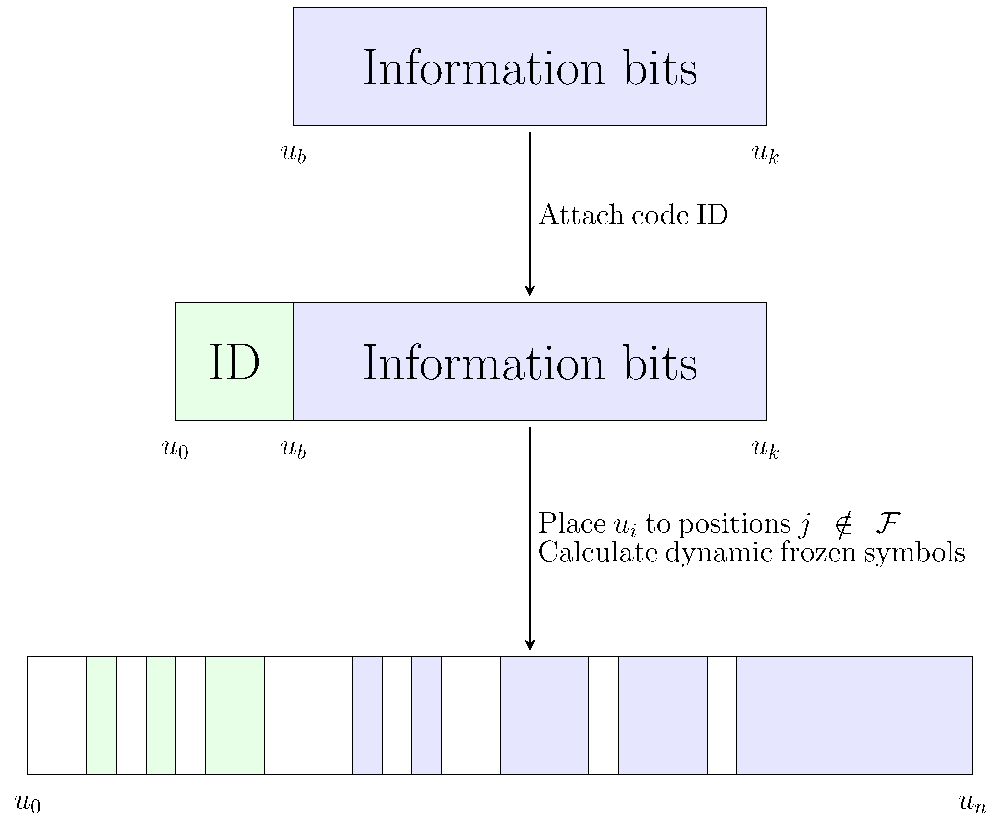
\includegraphics[width=0.45\textwidth]{./pictures/BlindStructure.eps}
  }\qquad
  \subfloat[Правая картинка]{
    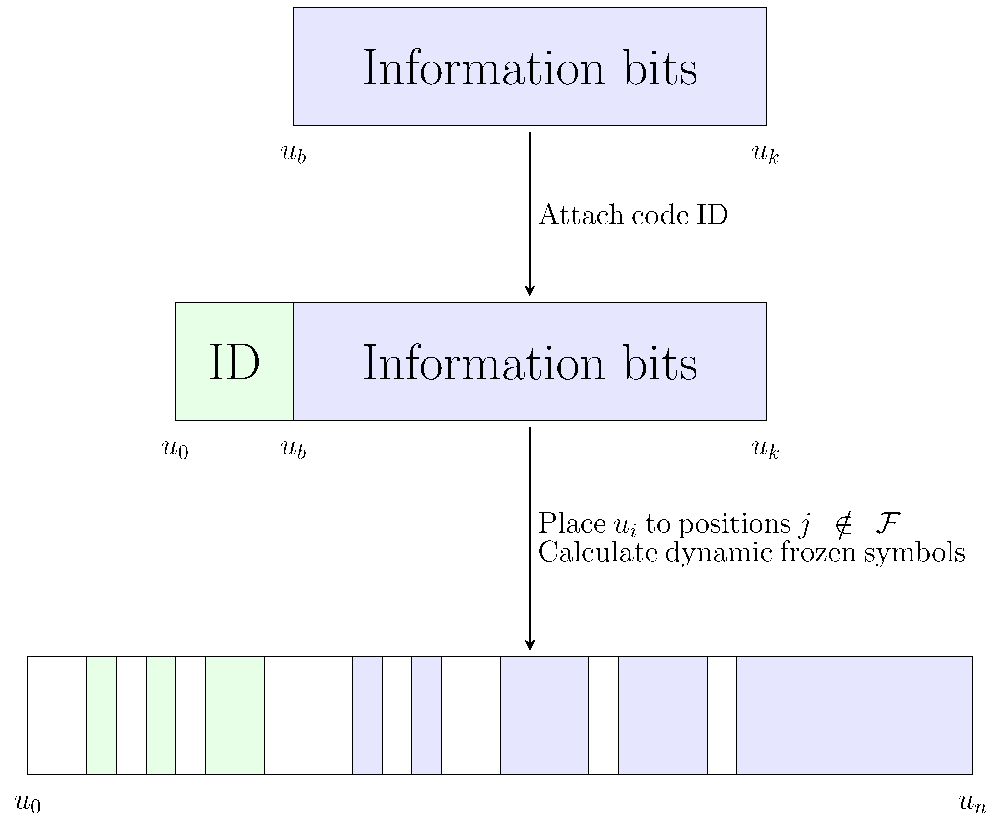
\includegraphics[width=0.45\textwidth]{./pictures/BlindStructure.eps}
  }
  \caption{Две одинаковых картинки}
  \label{2figs}
\end{figure}

%----------------------------------------------------------------------------------------
\subsection{hyperref, url}
Пакеты позволяют вставлять интерактивные ссылки в документ.
Примеры: 
\url{https://en.wikibooks.org/wiki/LaTeX/Hyperlinks},
\hyperlink{contents}{\contentsname}.

%----------------------------------------------------------------------------------------
\subsection{algorithm2e}
Пакет предоставляет вставлять в документ псевдокод алгоритмов.
В документе представлен алгоритм \ref{IR}.
% there is algorithm, function and procedure environments
\begin{procedure}
  % do not print semicolon at the end of each line
  \DontPrintSemicolon

  % define keywords, describing input and output parameters
  \SetKwInOut{Input}{input}
  \SetKwInOut{Output}{output}

  % describe variables
  \SetKwData{Left}{left}
  \SetKwData{This}{this}
  \SetKwData{Up}{up}

  % describe functions
  \SetKwFunction{Union}{Union}
  \SetKwFunction{FindCompress}{FindCompress}

  % begin of the algorithm description
  \Input{A bitmap $Im$ of size $w\times l$}
  \Output{A partition of the bitmap}
  \BlankLine

  \emph{текст на русском}\;
  еще текст на русском\;
  $i \leftarrow 2$\;
  \While{$i < l$}{
    \emph{special treatment of the first element of line $i$}\;
    \For{$j \leftarrow 2$ \KwTo $w$}{\label{forins}
      \Left $\leftarrow$ \FindCompress{$Im[i,j-1]$}\;
      \Up $\leftarrow$ \FindCompress{$Im[i-1,]$}\;
      \This $\leftarrow$ \FindCompress{$Im[i,j]$}\;

      \If(\tcp*[h]{O(\Left,\This)==1}){\Left compatible with \This}{\label{lt}
        \lIf{\Left $<$ \This}{\Union{\Left,\This}}
        \lElse{\Union{\This,\Left}}
      }

      \If(\tcp*[f]{O(\Up,\This)==1}){\Up compatible with \This}{\label{ut}
        \lIf{\Up $<$ \This}{\Union{\Up,\This}}
        \tcp{\This is put under \Up to keep tree as flat as possible}\label{cmt}
        \lElse{\Union{\This,\Up}}\tcp*[h]{\This linked to \Up}\label{lelse}
      }
    }
    \lForEach{element $e$ of the line $i$}{\FindCompress{p}}
  }

  \caption{IntervalRestriction($Im$)}
  \label{IR}
\end{procedure}


%----------------------------------------------------------------------------------------
\subsection{listings}
Пакет позволяет вставлять в текст листинги кода.
Пример кода C++ приведен на листинге \ref{l1}.

\begin{minipage}{\linewidth} % prevent page break inside listing
\begin{lstlisting}[caption={Hello,world!},label=l1]
  #include <iostream>
  int main() {
    std::cout << ``Hello, world!'' << std::endl;
    return 0;
  }
\end{lstlisting}
\end{minipage}

%----------------------------------------------------------------------------------------
\section{todonotes}
Пакет позволяет вставлять комментарии в документ, которые могут служить напоминанием при разработке большого документа.
\todo{Вставить ссылку}

Список всех комментариев может быть сформирован командой {\em listoftodos}.
\todo[inline]{Написать еще текста}

%----------------------------------------------------------------------------------------
%       BIBLIOGRAPHY
%----------------------------------------------------------------------------------------
\clearpage
\printbibliography

\listoftodos[TODO notes]
\end{document}
